% !TEX program = xelatex
\documentclass[10pt,letterpaper,twocolumn]{article}

\usepackage[top=0.75in, bottom=0.75in, left=0.75in, right=0.75in]{geometry}
\usepackage{fontspec}
\usepackage{unicode-math}
\setmainfont{Latin Modern Roman}[
  Extension=.otf,
  UprightFont=lmroman10-regular,
  BoldFont=lmroman10-bold,
  ItalicFont=lmroman10-italic,
  BoldItalicFont=lmroman10-bolditalic,
]
\setsansfont{Latin Modern Sans}[
  Extension=.otf,
  UprightFont=lmsans10-regular,
  BoldFont=lmsans10-bold,
  ItalicFont=lmsans10-oblique,
  BoldItalicFont=lmsans10-boldoblique,
]
\newfontfamily\acbold{ywft-processing-bold}[Path=../../system/public/type/webfonts/,Extension=.ttf]
\setmonofont{Latin Modern Mono}[
  Extension=.otf,
  UprightFont=lmmono10-regular,
  ItalicFont=lmmono10-italic,
  Scale=0.85,
]

\usepackage{xcolor}
\usepackage{titlesec}
\usepackage{enumitem}
\usepackage{booktabs}
\usepackage{tabularx}
\usepackage{fancyhdr}
\usepackage{hyperref}
\usepackage{xurl}
\usepackage{graphicx}
\graphicspath{{figures/}{../arxiv-ac/figures/}}
\usepackage{ragged2e}
\usepackage{microtype}
\usepackage{natbib}
\usepackage{tikz}
\usetikzlibrary{positioning,arrows.meta,calc}

\definecolor{acpink}{RGB}{180,72,135}
\definecolor{acpurple}{RGB}{120,80,180}
\definecolor{acdark}{RGB}{64,56,74}
\definecolor{acgray}{RGB}{119,119,119}

\hypersetup{colorlinks=true,linkcolor=acpurple,urlcolor=acpurple,citecolor=acpurple,
  pdftitle={Shipping the Easel},
  pdfauthor={Jeffrey Scudder}}

\titleformat{\section}{\normalfont\bfseries\normalsize\uppercase}{\thesection.}{0.5em}{}
\titlespacing{\section}{0pt}{1.2em}{0.3em}
\titleformat{\subsection}{\normalfont\bfseries\small}{\thesubsection}{0.5em}{}
\titlespacing{\subsection}{0pt}{0.8em}{0.2em}

\newcommand{\acdot}{{\color{acpink}.}}
\newcommand{\ac}{Aesthetic{\acdot}Computer}
\newcommand{\code}[1]{\texttt{#1}}

\pagestyle{fancy}\fancyhf{}
\renewcommand{\headrulewidth}{0pt}
\fancyhead[C]{\footnotesize\color{acpink}\textit{Field report --- \ac{} papers}}
\fancyfoot[C]{\footnotesize\thepage}

\setlist[itemize]{nosep, leftmargin=1.2em, itemsep=0.1em}
\setlist[enumerate]{nosep, leftmargin=1.4em, itemsep=0.1em}
\setlength{\columnsep}{1.8em}
\setlength{\parindent}{1em}
\setlength{\parskip}{0.3em}

\tolerance=800
\emergencystretch=1em
\hyphenpenalty=50

\begin{document}

\twocolumn[{%
\begin{center}

\includegraphics[height=4em]{pals}\par\vspace{0.5em}
{\acbold\fontsize{21pt}{25pt}\selectfont\color{acdark} Shipping the Easel}\par
\vspace{0.45em}
{\normalfont\itshape\fontsize{11pt}{13pt}\selectfont\color{acpink} What it would mean to hand someone else the editor, and the four things standing in the way}\par
\vspace{0.3em}
{\normalfont\fontsize{9pt}{11pt}\selectfont\color{acgray} Advertising is one act. Distributing, supporting, and paying for it are three others.}\par
\vspace{0.6em}
{\normalsize\href{https://prompt.ac/@jeffrey}{@jeffrey}}\par
{\small\color{acgray} \ac{} --- September 11, 2026}\par
{\small\color{acgray} ORCID: \href{https://orcid.org/0009-0007-4460-4913}{0009-0007-4460-4913}}\par
\vspace{0.3em}
{\small\color{acpurple} \url{https://aesthetic.computer}}\par
\vspace{0.6em}
\rule{\textwidth}{1.5pt}
\vspace{0.5em}
\end{center}

\begin{quote}
\small\noindent\textbf{Abstract.}
Easel is a 4{,}458-line terminal coding interface with no dependencies, 56
passing tests, and three days of history. It works. The question asked of it is
whether typing \code{easel} at the \ac{} prompt should now advertise a command-line
tool, and whether that tool should be shipped. This report separates four acts
that the word \emph{shipping} routinely conflates --- advertising, distributing,
supporting, and funding --- and finds that they have entirely different costs and
entirely different blockers. Advertising is a nine-line change to
\code{prompt.mjs} with an established pattern beside it. Distributing is blocked
outright: the licence reads \emph{all rights reserved}, and
\code{package.json} carries \code{private: true} with no \code{bin} field, so
\code{npm publish} would refuse before any policy question arose. Supporting is
constrained by a fact easy to miss from inside the fleet --- Easel is not
self-sufficient. It drives the \code{claude} or \code{codex} binary over stdio,
so a stranger who installs it and holds neither subscription gets a working
interface attached to nothing. Funding is, as of today, the one dimension
already solved: the identity gate and per-handle budget landed this morning, and
without them a distributed Easel would have pointed strangers at inference
\ac{} pays for. We recommend advertising now and distributing later, and give
the concrete shape of both. Registry facts are reported as measured: \code{easel}
is taken on npm by an unrelated package last touched in 2022, while
\code{ac-easel}, \code{aesthetic-easel}, and the \code{@aesthetic.computer} scope
are free.
\end{quote}
\vspace{0.5em}
}]

\section{The question}

Typing \code{easel} at the \ac{} prompt today does nothing. There is no piece by
that name, and the word falls through to the ordinary not-found path. The
proposal is that it should instead introduce the command-line tool of the same
name, and that the tool should be shipped.

Those are two requests, and the second one is four. This report takes them
apart, because they have different costs, different blockers, and --- the point
of separating them --- different answers.

\section{What is being shipped}

Easel is the terminal interface at \code{easel/} in this repository. It renders
its own conversation, streaming, tool activity, interruption, and approvals, and
drives an engine bridge --- a subprocess on stdio --- beneath that. Two bridges
ship: one speaking the headless Claude protocol, one speaking
\code{codex app-server}. It is 4{,}458 lines across sixteen modules with
\textbf{zero npm dependencies}, and 56 tests pass in under a second.

It is also three days old, and was a separate git repository with no remote
until this morning~\citep{scudder2026paying}. That is not an argument against
shipping it. It is context for how much of the surface below has ever been
exercised by anyone who is not its author.

\section{Four acts, not one}

\subsection{Advertise}

Make \code{easel} at the prompt say the tool exists. The pattern is already in
the codebase: \code{prompt.mjs} carries a branch for \code{menuband} that jumps
to an external URL, and neighbouring branches for \code{desktop}, \code{app},
and \code{electron}. An \code{easel} branch is the same shape.

This is cheap, reversible, and does not require any of the three acts below.
Crucially, it can point at a page that explains what Easel is and what it needs
--- including that it needs a vendor subscription --- without offering a
download at all.

\subsection{Distribute}

Put the code where a stranger can install it. This is blocked, twice.

\textbf{The licence.} \code{easel/LICENSE} reads \emph{all rights reserved}, and
grants no right to use, copy, modify, or distribute without prior written
permission. Publishing it anywhere public contradicts the file in its own
directory. This is a decision to make, not a bug to fix, but it must be made
before anything else in this subsection matters.

\textbf{The manifest.} \code{package.json} carries \code{"private": true}, which
makes \code{npm publish} refuse by design, and has no \code{bin} field, so
nothing would be linked onto a \code{PATH} even if it published~\citep{npmpublish}.
There is also
no \code{engines} floor recorded, though the code uses top-level \code{await}
and \code{node:test}.

\subsection{Support}

Be the place people arrive when it does not work. This is where the
least-visible constraint lives, and it is the one this report most wants to
surface.

\textbf{Easel is not self-sufficient.} Both bridges spawn a vendor binary ---
\code{claude} or \code{codex} --- and sign in with that vendor CLI's own
credentials, already on the machine. This is an elegant design from inside a
fleet where those binaries are always present. From outside, it means a stranger
who installs Easel and holds neither subscription gets a correct, well-tested,
attractively coloured interface attached to nothing at all.

The audience for Easel as it stands is therefore not ``people who want to make
pieces.'' It is the strictly smaller set of people who \emph{already pay
Anthropic or OpenAI} and would like a different editor in front of that
subscription. That set may be worth serving. It is not the set the word
\emph{shipping} usually implies, and the advertising copy has to say so in the
first sentence or the support burden is people reporting that nothing happens.

Table~\ref{tab:portability} records what else assumes the machine it was written
on.

\begin{table}[t]
\centering
\footnotesize
\begin{tabularx}{\columnwidth}{@{}lX@{}}
\toprule
\textbf{Assumption} & \textbf{Where, and what it costs} \\
\midrule
\code{/bin/ps} & \code{slab-session.mjs} reads the tty this way. BSD/macOS path; absent on many Linux images. \\
Slab markers & Sessions publish to \code{\~{}/.local/share/slab}. Harmless where absent, but dead code for everyone outside the fleet. \\
Openers & \code{open} / \code{xdg-open} / \code{start} are handled, so the browser login is portable. \\
Node floor & Unrecorded. Top-level \code{await} and \code{node:test} imply a modern runtime; nothing states which. \\
\bottomrule
\end{tabularx}
\caption{Portability surface. None of these is hard to fix; all of them are
currently untested off the fleet, because there has been nowhere else to run it.}
\label{tab:portability}
\end{table}

\subsection{Fund}

Pay for what the installed copies consume. This is the dimension that was
genuinely dangerous a day ago and is not any more.

A shipped Easel signs in through \ac{}'s Auth0 client and then talks to \ac{}'s
own endpoints: it publishes pieces under the user's handle, and it pushes source
to live code channels. Until this morning, \code{/api/ask} served any caller a
model of their choosing on \ac{}'s API keys, and \code{/run} accepted
unauthenticated writes to any channel~\citep{scudder2026paying}. Distributing a
CLI into that arrangement would have been an efficient way to convert a design
oversight into a bill.

Both are closed. Identity is resolved from a token, a handle receives a daily
budget that degrades rather than refuses, and channel ownership is a check
against the token rather than a secret in a name. The funding question for a
shipped Easel is now a matter of setting a number, not of building a mechanism
--- which is a real change in posture, and the reason this report can recommend
anything at all.

One note on identity: the Auth0 client embedded in \code{ac-session.mjs} is a
public PKCE client~\citep{oauthpkce} --- the kind designed to be embedded in
distributed software, because the proof of possession is generated per
authorisation rather than stored in the binary. It is already shared with
\code{ac-login}, the Slab menubar, the Xbox account flow, and the
Whistlegraph MCP. Shipping does not expose a secret. It does mean a stranger's
sign-in traverses the same client as internal tooling, which is worth knowing
before it is true rather than after.

\section{The shape of advertising, concretely}

Figure~\ref{fig:acts} orders the four acts by what each one requires of the
last.

\begin{figure}[t]
\centering
\footnotesize
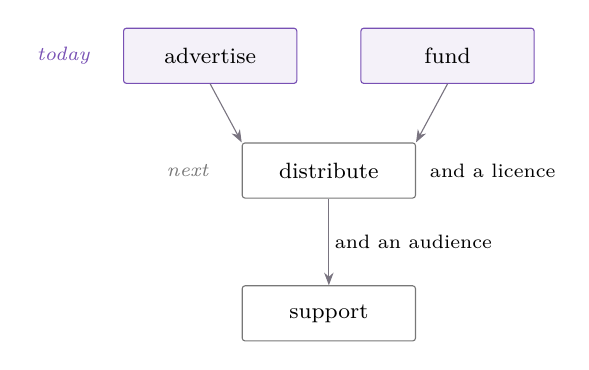
\begin{tikzpicture}[
  act/.style={draw=acdark, rounded corners=1pt, align=center, inner sep=4pt,
              minimum height=7mm, minimum width=22mm, font=\footnotesize},
  now/.style={act, draw=acpurple, fill=acpurple!8},
  later/.style={act, draw=acgray},
  line/.style={-{Stealth[length=1.6mm]}, draw=acdark!70},
  gate/.style={font=\scriptsize, inner sep=2pt, align=left},
]
\node[now] (adv) {advertise};
\node[now, right=8mm of adv] (fund) {fund};
\node[later, below=11mm of $(adv)!0.5!(fund)$] (dist) {distribute};
\node[later, below=11mm of dist] (sup) {support};

\draw[line] (adv.south) -- (dist.north west);
\draw[line] (fund.south) -- (dist.north east);
\draw[line] (dist) -- node[gate, right] {and an audience} (sup);
\node[gate, right=1mm of dist] {and a licence};

\node[font=\scriptsize\itshape, color=acpurple, left=3mm of adv] {today};
\node[font=\scriptsize\itshape, color=acgray, left=3mm of dist] {next};
\end{tikzpicture}
\caption{What each act rests on. The two in purple are available today ---
advertising needs nothing, and funding was settled this morning by the identity
gate and per-handle budget. Distribution rests on both of those \emph{and} on a
licence decision; support rests on distribution having found anyone at all.}
\label{fig:acts}
\end{figure}

If only the first is done, the work is: a branch in \code{prompt.mjs} beside the
\code{menuband} one, and a destination. The destination should state, in order,
what Easel is, that it requires a Claude or Codex subscription, and what it
does that a terminal does not --- the piece is live at a URL from the first
second, and the address is scannable from the prompt rock.

That page can honestly exist before any decision about distribution, and it is
the cheapest way to find out whether anyone wants this.

\section{If and when it is distributed}

Three routes, in ascending order of commitment.

\textbf{npm.} The conventional route for a Node CLI, and the one the artifact is
closest to: remove \code{private}, add \code{bin} and \code{engines}, publish.
The name \code{easel} is taken --- an unrelated package at version 0.2.6, last
modified in June 2022, whose description does not match its name. Squatted
names are occasionally recoverable through npm's dispute process, but the
cheaper answer is that \code{ac-easel} and \code{aesthetic-easel} are both free,
as is the \code{@aesthetic.computer} scope, which has the advantage of naming
the publisher in the install line.

\textbf{An install script served from \ac{}.} \code{curl | sh} is what most
terminal tools do, and \ac{} currently serves no shell script of any kind, so
this would be a new pattern rather than an extension of one. It also asks the
user to pipe a remote script into a shell, which is worth being deliberate
about rather than adopting because it is common.

\textbf{Homebrew.} A tap is the most macOS-native answer and the most
maintenance per release. Given the portability surface in
Table~\ref{tab:portability}, a macOS-first distribution is an honest match to
what is actually tested --- but it is also the route that forecloses the least.

Menu Band is the relevant precedent: it ships through the Mac App Store at
\$4.99, carries a version manifest, and counts its downloads through a backend
endpoint. That machinery exists and could be pointed at a second product
without inventing anything.

\section{Recommendation}

Advertise now; do not distribute yet.

Advertising costs a branch and a page, is reversible, requires no licence
decision, and answers the question that should be answered first --- whether
anyone outside this fleet wants a terminal editor whose output is a live URL.
The page should lead with the subscription requirement rather than bury it.

Before distributing, four things want doing, and only one of them is a judgement
call. Relicensing is the judgement call. The other three are small: add
\code{bin} and \code{engines} and drop \code{private}; replace the \code{/bin/ps}
tty lookup with something portable; and run the test suite once on a Linux
machine that has never seen this repository, which has not happened.

\section{Limitations}

This report is an audit of an artifact and a survey of options; it is not a
market estimate. We do not know whether anyone wants this, and nothing here
establishes that they do. The npm name availability was measured against the
registry today and can change. Whether the squatted \code{easel} package is
recoverable was not investigated beyond confirming it exists and is stale.

The portability claims are read from source, not from running Easel on another
operating system --- which is precisely the test that has not been performed,
and the one that would most cheaply de-risk any distribution decision.

\section{Conclusion}

The question was whether to advertise the CLI and ship it, and the useful answer
is that those were always two questions wearing one word.

Advertising is available now and blocked by nothing. Funding, which would have
been the serious objection a day ago, was settled this morning for unrelated
reasons. Distribution is blocked by a licence that says so in plain language
inside the directory being discussed, and that is a decision rather than an
obstacle. Support is constrained by the one fact most easily lost from inside a
fleet where every machine already has the vendor CLIs installed: Easel is a
beautiful front end to a subscription somebody else sells, and to a stranger
without one it does nothing at all.

That is not a reason to keep it private. It is the first sentence of the page
that advertises it.

\bibliographystyle{plainnat}
\bibliography{references}

\end{document}
